\documentclass [border=5pt, tikz]{standalone}
\usepackage[american,cuteinductors,smartlabels]{circuitikz}
\ctikzset{bipoles/thickness=1.2}
\ctikzset{bipoles/length=1cm}
\tikzstyle{every path}=[line width=0.8pt,line cap=round,line join=round]

\begin{document}
  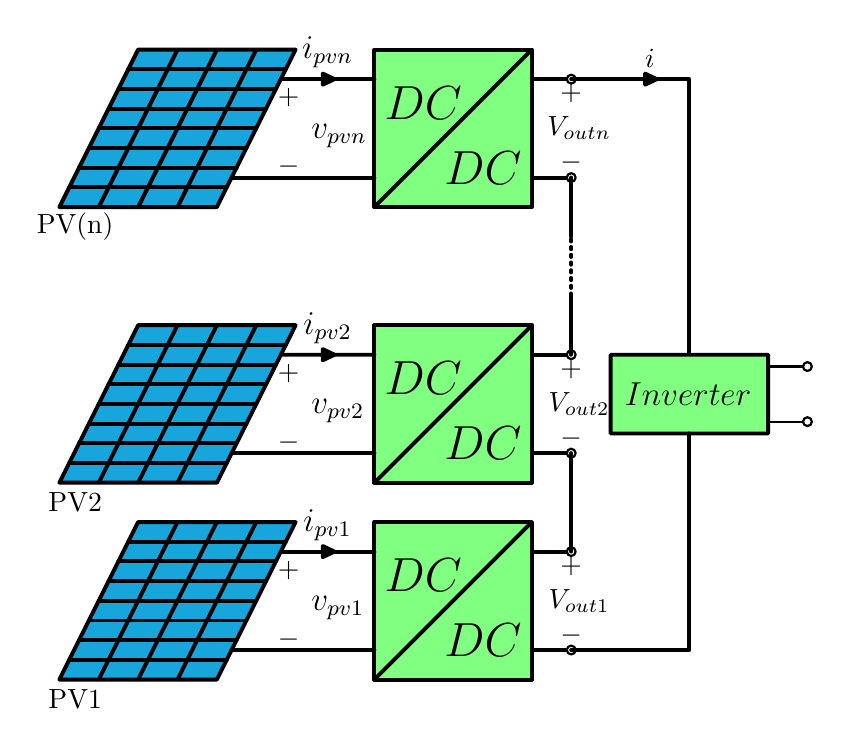
\begin{tikzpicture}
%------------- Part 1; Series (or cascaded) full power processing-------------------
%Panel1
	%Frame
	\draw (0,0) coordinate (P1);
	\draw (P1)++(2,0) coordinate(P2);
	\draw (P1)++(-1,-2) coordinate (P3);
	\draw (P3)++(2,0) coordinate(P4);
	\draw [line width=.5mm, fill=cyan!90!black] (P1)--(P2)--(P4)--(P3)--cycle;
	%Horizontal Lines
	\draw [line width=.5mm] (P1)++ (-.125,-0.25)--(1.875,-.25) ;
	\draw [line width=.5mm] (P1)++ (-.25,-0.5)--(1.75,-.5)  ;
	\draw [line width=.5mm] (P1)++ (-.375,-0.75)--(1.625,-.75) ;
	\draw [line width=.5mm] (P1)++ (-.5,-1)--(1.5,-1) ;
	\draw [line width=.5mm] (P1)++  (-.625,-1.25)--(1.375,-1.25) ;
	\draw [line width=.5mm] (P1)++ (-.75,-1.5)--++(2,0)  ;
	\draw [line width=.5mm] (P1)++  (-.875,-1.75)--++(2,0) coordinate (P34) ;
	%HVertical Line
	\draw [line width=.5mm] (.5,0)--++(-1,-2);
	\draw [line width=.5mm] (1,0)--++(-1,-2);
	\draw [line width=.5mm] (1.5,0)--++(-1,-2);
	\draw (P3)++(0.2,-0.25) coordinate (Pname);
	\node (PVname) at (Pname) {PV1};
	%Converter
	\draw [line width=.5mm] (P2)++(1,0) coordinate(C1);
	\draw (C1)++(2,0) coordinate (C2);
	\draw (C1)++(0,-2) coordinate (C3);
	\draw (C3)++(2,0) coordinate (C4);
	\draw  [line width=.5mm, fill=green!50] (C1)-- (C3)--(C4)--(C2)--cycle;
	\draw [line width=.5mm] (C3)--(C2);
	%
	\draw (1.8125,-.375)  coordinate(conn1) ;
	\draw (P4)++(.125,.25)--++(.0625,.125) coordinate(conn2) ;
	\draw (conn1)++(.1,-.05) coordinate(VPV);
	%Connection of Panel and coverter
	\draw (conn1-|C1) coordinate(connC1);
	\draw (conn2-|C1) coordinate(connC2);
	\draw (conn1)--++(1,0);
	\draw [line width=.5mm] (conn1) to [short,i=\large$i_{pv1}$](connC1);
	\draw (VPV) to [open, l=\large$ v_{pv1}$, v^=$$]++(0,-1.25);
	\draw [line width=.5mm] (conn2) --(connC2);
	%
	\draw (connC1)++(2,0) coordinate (connC3);
	\draw (connC2)++(2,0) coordinate (connC4);
	%
	\draw (C2)++(0,-1) coordinate (CM); %middle of converter at right side
	\draw (CM)++(0.6,0) node (Vot){$V_{out1}$};
	\draw [line width=.5mm] (connC3)--++(0.5,0) coordinate(OutUp1);
	\draw [line width=.5mm] (connC4)--++(0.5,0) coordinate(OutBt1);
	\draw  (OutUp1) to [open,o-o, v=$$](OutBt1);
	%
	\draw (connC1)++(0,-.3) coordinate (T1);
	\node [below, right](Text1) at (T1) {\LARGE $DC$}; 
	\draw (C4)++(0,0.5) coordinate (T2);
	\node [above, left](Text1) at (T2) {\LARGE$ DC$}; 

%Panel2
	%Frame
	\draw (0,2.5) coordinate (P1-2);
	\draw (P1-2)++(2,0) coordinate(P2-2);
	\draw (P1-2)++(-1,-2) coordinate (P3-2);
	\draw (P3-2)++(2,0) coordinate(P4-2);
	\draw [line width=.5mm, fill=cyan!90!black] (P1-2)--(P2-2)--(P4-2)--(P3-2)--cycle;
	%Horizontal Lines
	\draw [line width=.5mm] (P1-2)++ (-.125,-0.25)--++(2,0) ;
	\draw [line width=.5mm] (P1-2)++ (-.25,-0.5)--++(2,0)   ;
	\draw [line width=.5mm] (P1-2)++ (-.375,-0.75)--++(2,0)  ;
	\draw [line width=.5mm] (P1-2)++ (-.5,-1)--++(2,0)  ;
	\draw [line width=.5mm] (P1-2)++  (-.625,-1.25)--++(2,0)  ;
	\draw [line width=.5mm] (P1-2)++ (-.75,-1.5)--++(2,0)  ;
	\draw [line width=.5mm] (P1-2)++  (-.875,-1.75)--++(2,0) coordinate (P34-2) ;
	%Vertical Line
	\draw [line width=.5mm] (P1-2)++(.5,0)--++(-1,-2);
	\draw [line width=.5mm](P1-2)++ (1,0)--++(-1,-2);
	\draw [line width=.5mm] (P1-2)++(1.5,0)--++(-1,-2);
	\draw (P3-2)++(0.2,-0.25) coordinate (Pname-2);
	\node (PVname-2) at (Pname-2) {PV2};
	%Converter
	\draw [line width=.5mm] (P2-2)++(1,0) coordinate(C1-2);
	\draw (C1-2)++(2,0) coordinate (C2-2);
	\draw (C1-2)++(0,-2) coordinate (C3-2);
	\draw (C3-2)++(2,0) coordinate (C4-2);
	\draw  [line width=.5mm, fill=green!50] (C1-2)-- (C3-2)--(C4-2)--(C2-2)--cycle;
	\draw [line width=.5mm] (C3-2)--(C2-2);
	%
	\draw (P1-2)++ (1.8125,-.375)  coordinate(conn12) ;
	\draw (P4-2)++(.125,.25)--++(.0625,.125) coordinate(conn22) ;
	\draw (conn12)++(.1,-.05) coordinate(VPV-2);
	% Connection of Panel and coverter
	\draw (conn12-|C1-2) coordinate(connC1-2);
	\draw (conn22-|C1-2) coordinate(connC2-2);
	\draw (conn12)--++(1,0);
	\draw [line width=.5mm] (conn12) to [short,i=\large$i_{pv2}$](connC1-2);
	\draw (VPV-2) to [open, l=\large$ v_{pv2}$, v^=$$]++(0,-1.25);
	\draw [line width=.5mm] (conn22) --(connC2-2);
	%
	\draw (connC1-2)++(2,0) coordinate (connC3-2);
	\draw (connC2-2)++(2,0) coordinate (connC4-2);
	%
	\draw (C2-2)++(0,-1) coordinate (CM2); %middle of converter at right side
	\draw (CM2)++(.6,0) node (Vot2){$V_{out2}$};
	\draw [line width=.5mm] (connC3-2)--++(0.5,0) coordinate(OutUp2);
	\draw [line width=.5mm] (connC4-2)--++(0.5,0) coordinate(OutBt2);
	\draw  (OutUp2) to [open,o-o, v=$$](OutBt2);
	\draw (connC1-2)++(0,-.3) coordinate (T1-2);
	\node [below, right](Text1-2) at (T1-2) {\LARGE $DC$}; 
	\draw (C4-2)++(0,0.5) coordinate (T2-2);
	\node [above, left](Text1-2) at (T2-2) {\LARGE$ DC$}; 

%Panel3
	%Frame
	\draw (0,6) coordinate (P1-3);
	\draw (P1-3)++(2,0) coordinate(P2-3);
	\draw (P1-3)++(-1,-2) coordinate (P3-3);
	\draw (P3-3)++(2,0) coordinate(P4-3);
	\draw [line width=.5mm, fill=cyan!90!black] (P1-3)--(P2-3)--(P4-3)--(P3-3)--cycle;
	%Horizontal Lines
	\draw [line width=.5mm] (P1-3)++ (-.125,-0.25)--++(2,0) ;
	\draw [line width=.5mm] (P1-3)++ (-.25,-0.5)--++(2,0)   ;
	\draw [line width=.5mm] (P1-3)++ (-.375,-0.75)--++(2,0)  ;
	\draw [line width=.5mm] (P1-3)++ (-.5,-1)--++(2,0)  ;
	\draw [line width=.5mm] (P1-3)++  (-.625,-1.25)--++(2,0)  ;
	\draw [line width=.5mm] (P1-3)++ (-.75,-1.5)--++(2,0)  ;
	\draw [line width=.5mm] (P1-3)++  (-.875,-1.75)--++(2,0) coordinate (P34-3) ;
	%Vertical Line-
	\draw [line width=.5mm] (P1-3)++(.5,0)--++(-1,-2);
	\draw [line width=.5mm](P1-3)++ (1,0)--++(-1,-2);
	\draw [line width=.5mm] (P1-3)++(1.5,0)--++(-1,-2);
	\draw (P3-3)++(0.2,-0.25) coordinate (Pname-3);
	\node (PVname-3) at (Pname-3) {PV(n)};
	%Converte
	\draw [line width=.5mm] (P2-3)++(1,0) coordinate(C1-3);
	\draw (C1-3)++(2,0) coordinate (C2-3);
	\draw (C1-3)++(0,-2) coordinate (C3-3);
	\draw (C3-3)++(2,0) coordinate (C4-3);
	\draw  [line width=.5mm, fill=green!50] (C1-3)-- (C3-3)--(C4-3)--(C2-3)--cycle;
	\draw [line width=.5mm] (C3-3)--(C2-3);
	\draw (P1-3)++ (1.8125,-.375)  coordinate(conn13) ;
	\draw (P4-3)++(.125,.25)--++(.0625,.125) coordinate(conn23) ;
	\draw (conn13)++(.1,-.05) coordinate(VPV-3);
	%Connection of Panel and coverter
	\draw (conn13-|C1-3) coordinate(connC1-3);
	\draw (conn23-|C1-3) coordinate(connC2-3);
	\draw (conn13)--++(1,0);
	\draw [line width=.5mm] (conn13) to [short,i=\large$i_{pvn}$](connC1-3);
	\draw (VPV-3) to [open, l=\large$ v_{pvn}$, v^=$$]++(0,-1.25);
	\draw [line width=.5mm] (conn23) --(connC2-3);
	%
	\draw (connC1-3)++(2,0) coordinate (connC3-3);
	\draw (connC2-3)++(2,0) coordinate (connC4-3);
	%
	\draw (C2-3)++(0,-1) coordinate (CM3); %middle of converter at right side
	\draw (CM3)++(.6,0) node (Vot3){$V_{outn}$};
	\draw [line width=.5mm] (connC3-3)--++(0.5,0) coordinate(OutUp3);
	\draw [line width=.5mm] (connC4-3)--++(0.5,0) coordinate(OutBt3);
	\draw  (OutUp3) to [open,o-o, v=$$](OutBt3);
	\draw (connC1-3)++(0,-.3) coordinate (T1-3);
	\node [below, right](Text1-3) at (T1-3) {\LARGE $DC$}; 
	\draw (C4-3)++(0,0.5) coordinate (T2-3);
	\node [above, left](Text1-3) at (T2-3) {\LARGE$ DC$}; 
	%Connections
	\draw [line width=.5mm](OutUp1)--(OutBt2);
	\draw [line width=.5mm] (OutUp2) --++(0,0.75) coordinate (Line1);
	\draw [dotted, line width=.5mm](Line1)--++(0,0.75) coordinate (Line2);
	\draw [line width=.5mm] (Line2)--(OutBt3);

%Inverter
	\draw [line width=.5mm] (OutUp3) --++(0.5,0) to [short,i=$i$]++(1,0)--++(0,-3.5) coordinate(CMu);
	\draw (CMu)++(-1,-.5) coordinate (CMl);
	\draw (CMl)++(1,-.5) coordinate (CMb);
	\draw (CMb)++(1,0.15) coordinate (CO2);
	\draw (CO2)++(0,0.7) coordinate (CO1);
	\draw [line width=.5mm, fill=green!50] (CMu)--++(-1,0)--(CMl)-- ++(0,-0.5)--(CMb)--++(1,0)--(CO2)--(CO1)--++(0,0.15)--cycle;
	\draw [line width=.5mm] (OutBt1)--++(1.5,0)--(CMb);
	\draw (CMl)++(.05,0) coordinate (CMl1);
	\node [right] (Conv) at (CMl1) {\large $Inverter$};
	% Inverter's AC output
	\draw (CO1)--++(0.5,0) to [open,o-o]++(0,-0.7)--(CO2);

  \end{tikzpicture}

%------------- Part 2; Parallel full power processing-------------------
  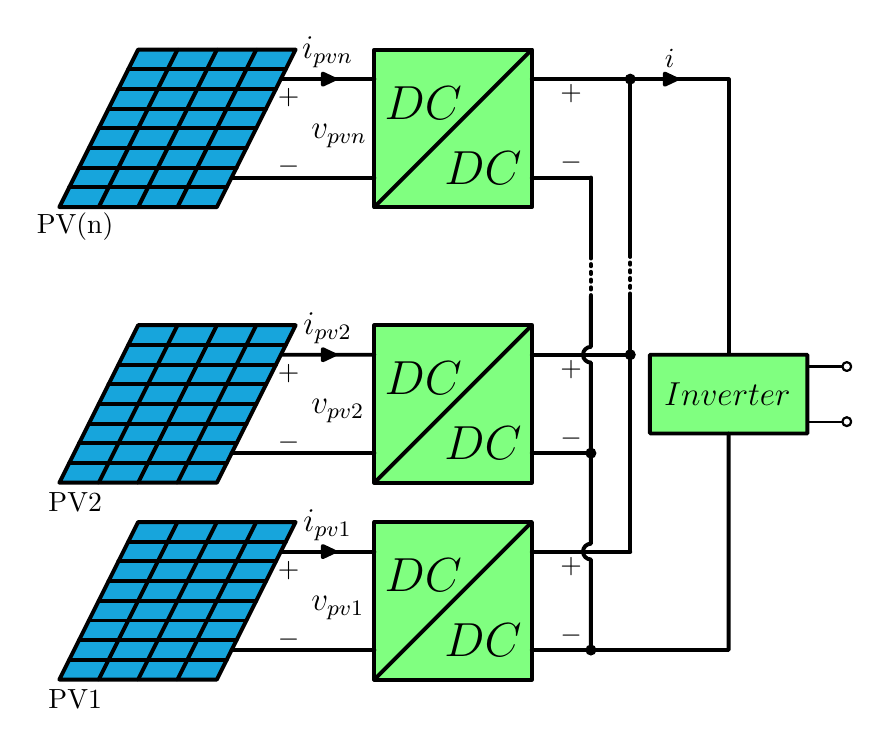
\begin{tikzpicture}
%-Panel1
	%Frame
	\draw (0,0) coordinate (P1);
	\draw (P1)++(2,0) coordinate(P2);
	\draw (P1)++(-1,-2) coordinate (P3);
	\draw (P3)++(2,0) coordinate(P4);
	\draw [line width=.5mm, fill=cyan!90!black] (P1)--(P2)--(P4)--(P3)--cycle;
	%Horizontal Lines
	\draw [line width=.5mm] (P1)++ (-.125,-0.25)--(1.875,-.25) ;
	\draw [line width=.5mm] (P1)++ (-.25,-0.5)--(1.75,-.5)  ;
	\draw [line width=.5mm] (P1)++ (-.375,-0.75)--(1.625,-.75) ;
	\draw [line width=.5mm] (P1)++ (-.5,-1)--(1.5,-1) ;
	\draw [line width=.5mm] (P1)++  (-.625,-1.25)--(1.375,-1.25) ;
	\draw [line width=.5mm] (P1)++ (-.75,-1.5)--++(2,0)  ;
	\draw [line width=.5mm] (P1)++  (-.875,-1.75)--++(2,0) coordinate (P34) ;
	%%HVertical Line
	\draw [line width=.5mm] (.5,0)--++(-1,-2);
	\draw [line width=.5mm] (1,0)--++(-1,-2);
	\draw [line width=.5mm] (1.5,0)--++(-1,-2);
	\draw (P3)++(0.2,-0.25) coordinate (Pname);
	\node (PVname) at (Pname) {PV1};
	%Converter
	\draw [line width=.5mm] (P2)++(1,0) coordinate(C1);
	\draw (C1)++(2,0) coordinate (C2);
	\draw (C1)++(0,-2) coordinate (C3);
	\draw (C3)++(2,0) coordinate (C4);
	\draw  [line width=.5mm, fill=green!50] (C1)-- (C3)--(C4)--(C2)--cycle;
	\draw [line width=.5mm] (C3)--(C2);
	%
	\draw (1.8125,-.375)  coordinate(conn1) ;
	\draw (P4)++(.125,.25)--++(.0625,.125) coordinate(conn2) ;
	\draw (conn1)++(.1,-.05) coordinate(VPV);
	
	%Connection of Panel and coverter
	%
	\draw (conn1-|C1) coordinate(connC1);
	\draw (conn2-|C1) coordinate(connC2);
	\draw (conn1)--++(1,0);
	\draw [line width=.5mm] (conn1) to [short,i=\large$i_{pv1}$](connC1);
	\draw (VPV) to [open, l=\large$ v_{pv1}$, v^=$$]++(0,-1.25);
	\draw [line width=.5mm] (conn2) --(connC2);
	
	
	%######
	\draw (connC1)++(2,0) coordinate (connC3);
	\draw (connC2)++(2,0) coordinate (connC4);
	%
	\draw (C2)++(0,-1) coordinate (CM); %middle of converter at right side
	%parallell
	\draw [line width=.5mm] (connC3)--++(0.5,0) coordinate(OutUp1)--++(0.75,0) coordinate(OutParallel1u);
	\draw [line width=.5mm] (connC4)--++(0.5,0) coordinate(OutBt1)--++(0.25,0) coordinate (OutParallel1b);
	\fill (OutParallel1b) circle (2pt);
	\draw  (OutUp1) to [open, v=$$](OutBt1);
	\draw (connC1)++(0,-.3) coordinate (T1);
	\node [below, right](Text1) at (T1) {\LARGE $DC$}; 
	\draw (C4)++(0,0.5) coordinate (T2);
	\node [above, left](Text1) at (T2) {\LARGE$ DC$}; 

%Panel2
	%Frame
	\draw (0,2.5) coordinate (P1-2);
	\draw (P1-2)++(2,0) coordinate(P2-2);
	\draw (P1-2)++(-1,-2) coordinate (P3-2);
	\draw (P3-2)++(2,0) coordinate(P4-2);
	\draw [line width=.5mm, fill=cyan!90!black] (P1-2)--(P2-2)--(P4-2)--(P3-2)--cycle;
	%Horizontal Lines
	\draw [line width=.5mm] (P1-2)++ (-.125,-0.25)--++(2,0) ;
	\draw [line width=.5mm] (P1-2)++ (-.25,-0.5)--++(2,0)   ;
	\draw [line width=.5mm] (P1-2)++ (-.375,-0.75)--++(2,0)  ;
	\draw [line width=.5mm] (P1-2)++ (-.5,-1)--++(2,0)  ;
	\draw [line width=.5mm] (P1-2)++  (-.625,-1.25)--++(2,0)  ;
	\draw [line width=.5mm] (P1-2)++ (-.75,-1.5)--++(2,0)  ;
	\draw [line width=.5mm] (P1-2)++  (-.875,-1.75)--++(2,0) coordinate (P34-2) ;
	%Vertical Line
	\draw [line width=.5mm] (P1-2)++(.5,0)--++(-1,-2);
	\draw [line width=.5mm](P1-2)++ (1,0)--++(-1,-2);
	\draw [line width=.5mm] (P1-2)++(1.5,0)--++(-1,-2);
	\draw (P3-2)++(0.2,-0.25) coordinate (Pname-2);
	\node (PVname-2) at (Pname-2) {PV2};
	%Converter
	\draw [line width=.5mm] (P2-2)++(1,0) coordinate(C1-2);
	\draw (C1-2)++(2,0) coordinate (C2-2);
	\draw (C1-2)++(0,-2) coordinate (C3-2);
	\draw (C3-2)++(2,0) coordinate (C4-2);
	\draw  [line width=.5mm, fill=green!50] (C1-2)-- (C3-2)--(C4-2)--(C2-2)--cycle;
	\draw [line width=.5mm] (C3-2)--(C2-2);
	%
	\draw (P1-2)++ (1.8125,-.375)  coordinate(conn12) ;
	\draw (P4-2)++(.125,.25)--++(.0625,.125) coordinate(conn22) ;
	\draw (conn12)++(.1,-.05) coordinate(VPV-2);
	%Connection of Panel and coverter
	\draw (conn12-|C1-2) coordinate(connC1-2);
	\draw (conn22-|C1-2) coordinate(connC2-2);
	\draw (conn12)--++(1,0);
	\draw [line width=.5mm] (conn12) to [short,i=\large$i_{pv2}$](connC1-2);
	\draw (VPV-2) to [open, l=\large$ v_{pv2}$, v^=$$]++(0,-1.25);
	\draw [line width=.5mm] (conn22) --(connC2-2);
	%
	\draw (connC1-2)++(2,0) coordinate (connC3-2);
	\draw (connC2-2)++(2,0) coordinate (connC4-2);
	%
	\draw (C2-2)++(0,-1) coordinate (CM2); %middle of converter at right side
	%parallell
	\draw [line width=.5mm] (connC3-2)--++(0.5,0) coordinate(OutUp2)--++(0.75,0)coordinate(OutParallel2u);
	\fill (OutParallel2u) circle (2pt);
	\draw [line width=.5mm] (connC4-2)--++(0.5,0) coordinate(OutBt2)--++(0.25,0) coordinate (OutParallel2b);
	\fill (OutParallel2b) circle (2pt);
	\draw  (OutUp2) to [open,v=$$](OutBt2);
	%
	\draw (connC1-2)++(0,-.3) coordinate (T1-2);
	\node [below, right](Text1-2) at (T1-2) {\LARGE $DC$}; 
	\draw (C4-2)++(0,0.5) coordinate (T2-2);
	\node [above, left](Text1-2) at (T2-2) {\LARGE$ DC$}; 

%Panel3
	%Frame
	\draw (0,6) coordinate (P1-3);
	\draw (P1-3)++(2,0) coordinate(P2-3);
	\draw (P1-3)++(-1,-2) coordinate (P3-3);
	\draw (P3-3)++(2,0) coordinate(P4-3);
	\draw [line width=.5mm, fill=cyan!90!black] (P1-3)--(P2-3)--(P4-3)--(P3-3)--cycle;
	%Horizontal Lines
	\draw [line width=.5mm] (P1-3)++ (-.125,-0.25)--++(2,0) ;
	\draw [line width=.5mm] (P1-3)++ (-.25,-0.5)--++(2,0)   ;
	\draw [line width=.5mm] (P1-3)++ (-.375,-0.75)--++(2,0)  ;
	\draw [line width=.5mm] (P1-3)++ (-.5,-1)--++(2,0)  ;
	\draw [line width=.5mm] (P1-3)++  (-.625,-1.25)--++(2,0)  ;
	\draw [line width=.5mm] (P1-3)++ (-.75,-1.5)--++(2,0)  ;
	\draw [line width=.5mm] (P1-3)++  (-.875,-1.75)--++(2,0) coordinate (P34-3) ;
	%Vertical Line
	\draw [line width=.5mm] (P1-3)++(.5,0)--++(-1,-2);
	\draw [line width=.5mm](P1-3)++ (1,0)--++(-1,-2);
	\draw [line width=.5mm] (P1-3)++(1.5,0)--++(-1,-2);
	\draw (P3-3)++(0.2,-0.25) coordinate (Pname-3);
	\node (PVname-3) at (Pname-3) {PV(n)};
	%Converter
	\draw [line width=.5mm] (P2-3)++(1,0) coordinate(C1-3);
	\draw (C1-3)++(2,0) coordinate (C2-3);
	\draw (C1-3)++(0,-2) coordinate (C3-3);
	\draw (C3-3)++(2,0) coordinate (C4-3);
	\draw  [line width=.5mm, fill=green!50] (C1-3)-- (C3-3)--(C4-3)--(C2-3)--cycle;
	\draw [line width=.5mm] (C3-3)--(C2-3);
	%
	\draw (P1-3)++ (1.8125,-.375)  coordinate(conn13) ;
	\draw (P4-3)++(.125,.25)--++(.0625,.125) coordinate(conn23) ;
	\draw (conn13)++(.1,-.05) coordinate(VPV-3);
	%Connection of Panel and coverter
	\draw (conn13-|C1-3) coordinate(connC1-3);
	\draw (conn23-|C1-3) coordinate(connC2-3);
	\draw (conn13)--++(1,0);
	\draw [line width=.5mm] (conn13) to [short,i=\large$i_{pvn}$](connC1-3);
	\draw (VPV-3) to [open, l=\large$ v_{pvn}$, v^=$$]++(0,-1.25);
	\draw [line width=.5mm] (conn23) --(connC2-3);
	%
	\draw (connC1-3)++(2,0) coordinate (connC3-3);
	\draw (connC2-3)++(2,0) coordinate (connC4-3);
	%
	\draw (C2-3)++(0,-1) coordinate (CM3); %middle of converter at right side
	%parallell
	\draw [line width=.5mm] (connC3-3)--++(0.5,0) coordinate(OutUp3)--++(0.75,0)coordinate(OutParallel3u);
	\fill (OutParallel3u) circle (2pt);
	\draw [line width=.5mm] (connC4-3)--++(0.5,0) coordinate(OutBt3)--++(0.25,0) coordinate (OutParallel3b);
	\draw  (OutUp3) to [open,v=$$](OutBt3);
	\draw (connC1-3)++(0,-.3) coordinate (T1-3);
	\node [below, right](Text1-3) at (T1-3) {\LARGE $DC$}; 
	\draw (C4-3)++(0,0.5) coordinate (T2-3);
	\node [above, left](Text1-3) at (T2-3) {\LARGE$ DC$}; 

	%Connections
	\draw [line width=.5mm] (OutParallel1u)--(OutParallel2u)--++(0,0.75) coordinate (dashp1);
	\draw  [dotted, line width=.5mm]  (dashp1)--++(0,0.5) coordinate (dashp2);
	\draw  [line width=.5mm] (dashp2)--(OutParallel3u);
	\draw [line width=.5mm] (OutParallel3b)--++(0,-1) coordinate (dashn1);
	\draw [dotted, line width=.5mm] (dashn1)--++(0,-0.5) coordinate (dashn2);
	\draw [line width=.5mm] (dashn2)--++(0,-0.65) arc (90:270:0.1)--(OutParallel2b)--++(0,-1.15) arc (90:270:0.1)--(OutParallel1b) ;

%Inverter
	\draw [line width=.5mm] (OutUp3) --++(0.5,0) to [short,i=$i$]++(1.5,0)--++(0,-3.5) coordinate(CMu);
	\draw (CMu)++(-1,-.5) coordinate (CMl);
	\draw (CMl)++(1,-.5) coordinate (CMb);
	\draw (CMb)++(1,0.15) coordinate (CO2);
	\draw (CO2)++(0,0.7) coordinate (CO1);
	\draw [line width=.5mm, fill=green!50] (CMu)--++(-1,0)--(CMl)-- ++(0,-0.5)--(CMb)--++(1,0)--(CO2)--(CO1)--++(0,0.15)--cycle;
	\draw [line width=.5mm] (OutBt1)--++(2,0)--(CMb);
	\draw (CMl)++(.05,0) coordinate (CMl1);
	\node [right] (Conv) at (CMl1) {\large $Inverter$};
	%Inverter's AC outputs
	\draw (CO1)--++(0.5,0) to [open,o-o]++(0,-0.7)--(CO2);
\end{tikzpicture}

\end{document}